\documentclass{article}

\usepackage{../preamble}
\standalonetrue

\pagestyle{fancy}
\fancyhf{}
\rhead{Section \thesection}
\lhead{PHYS 304 Lecture 23}
\rfoot{Page \thepage}


\title{PHYS 304 Lecture 23}
\author{Ashtan Mistal}
\date{!!!}

\begin{document}

\ifstandalone
\maketitle
\fi

\graphicspath{{./Lecture23/}}

\section{Review of key points from last lecture}

% - find slides

Using only the commutation relations between the various angular momentum operators, $\hat{L}_x, \hat{L}_y, \hat{L}_z, \hat{L}^2, \hat{L}_+, \hat{L}_-$ along with the physical interpretation of the observable operators, it is possible to deduce the entire spectrum of possible shared eigen values of $\hat{L}^2$  and one of the components of the angular momentum,  $\hat{L}_z$ using only Dirac notation (i.e. without the need to find any eigen functions)!  
The result is that the allowed eigen values of $\hat{L}^2$ are $\hbar^2 l (l+1)$, where $l$ must be zero or a positive half or full integer, and for a given value of $l$, the corresponding eigen values of the $2l+1$ degenerate eigen states of $\hat{L}_z$ are $\hbar m$, where $m  -l, =l+1,...,l$. 


It turns out that the equations that define the eigen functions for $\widehat{L^{2}}$, and $\widehat{L_{z}}$ in the 3D real space basis, $|\vec{r}\rangle$, using spherical coordinates, are identical to the "angular equations" that we solved when finding the stationary states of an electron in a spherically symmetric potential. Their solutions are therefore the spherical harmonic functions $Y_{l}^{m}(\theta, \phi)$. The $e^{i m \phi}$ contributions to each spherical harmonic function are directly traceable to the eigen functions of $\widehat{L}_{z}$, which is an operator that in the position basis depends only on $\phi .$

Therefore the shared eigen functions of $\hat{L^{2}}$, and $\hat{L_{z}}$ in the 3D real space basis, are precisely the spherical harmonics, $Y_{l}^{m}(\theta, \phi)$, with respective eigen values $\hbar^{2} l(l+1)$, and $m=$ $-l,-l+1, \ldots l$. The only difference between these sets of eigen functions and eigen values as compared to the stationary states of the electron in a spherically symmetric potential, is that in the latter case, $l$ is restricted to having values $0,1,2 \ldots$, whereas more generally, $l$ can take on values $0, \frac{1}{2}, 1, \frac{3}{2}, 2, \ldots$

\section{Today: Intrinsic Spin}

\subsection{Why no half integer l values in our hydrogen atom solutions?}

\begin{quote}
    “Our spherical harmonics, $Y_l^m (\theta, \phi)$ are nothing other than the (already normalized) common eigen functions of the  $\hat{L}^2$ and the $\hat{L}_z$ operators in the position basis, in spherical coordinates, but only including non-negative integer, not half-integer values of $l$” 
\end{quote}

The restriction to only integer values of $l$ arose because …. ?

\begin{itemize}
    \item Because we forced the associated wavefunctions, in the position basis, to be single-valued at all positions (in particular all values of $\phi$, modulo $2 \pi$). 
    \item Did we screw up, are their also solutions of our simple hydrogen atom Hamiltonian that have half integer values of $l$ and $m$?
\end{itemize}

No, the result is experimentally correct, validating the assumption of the single-valued nature of position space wavefunctions.  Then did we screw up in the derivation of the general spectrum?

Apparently not!

\subsection{Electron Spin}

If there was an measurement apparatus that could deflect a stream of incident atoms upwards or downwards an amount proportional to the z component of their angular momentum, sketch what would you expect to see on a screen that imaged the particles coming out the other side when hydrogen atoms are incident in state i) $\psi_{1,0,0},$ ii) $\psi_{2,1,0}$, iii) $\psi_{2,1,1}$, and iv) $\psi_{2,1,-1}$. 

Upwards in proportion to $\hbar$


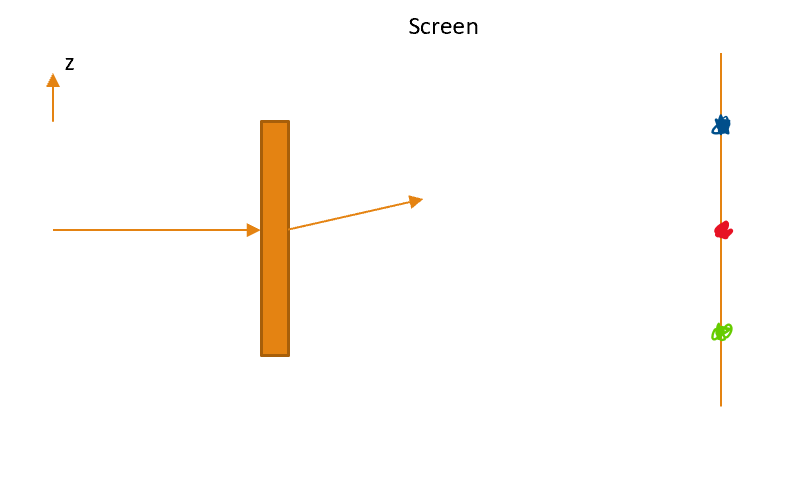
\includegraphics[width = 0.7 \textwidth]{Lecture23/1.png}

% on slide 7


\section{Electron Spin}

It turns out that if you send a beam of hydrogen atoms in the $\psi_{1,0,0}$ state through such an apparatus, there are two spots on the screen corresponding to an upward and downward deflection one would expect for a particle having an angular momentum $\pm \frac{\hbar}{2}$.  What are the implications of this observation? 

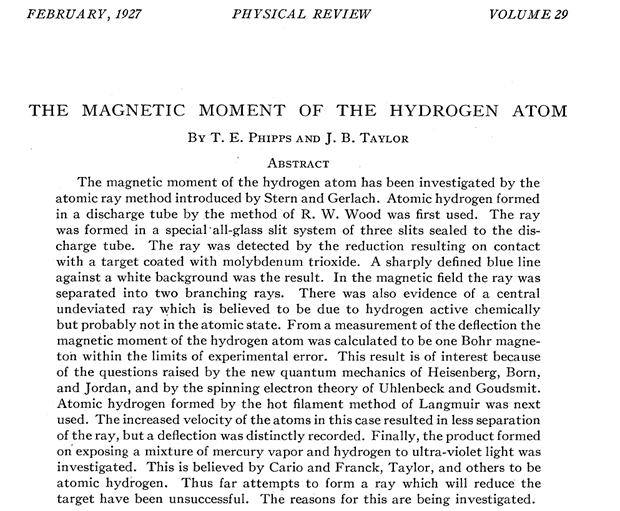
\includegraphics[width = 0.7 \textwidth]{Lecture23/2.png}

\begin{itemize}
    \item Point-like particle possesses "intrinsic" angular momentum quantized in units of $\frac{\hbar}{2}$, independent of position, linear or angular orbital momentum of the electron. 
    
    \item This spin degree of freedom must exist in some \textbf{separate Hilbert space}. It makes no sense to project its "spin state"  onto position or momentum basis states. What \textit{is} its nature then?
    
    \item Clearly associated with angular momentum, appears to behave like an entity that has two possible eigen values of a Cartesian component of angular momentum, $m = \pm \frac{\hbar}{2}$ -- Finally a justification for all that Dirac notation!
\end{itemize}


The electron must possess an “intrinsic” angular momentum, regardless of it’s “motion in space”…hence the term spin.

As far as we know, the electron is a fundamental quantum mechanical property with no measurable (or measured) intrinsic size.  As we have learned, quantum mechanics associates a probability distribution for where this infinitely small particle might be observed when it is in some given QM state, but the particle itself has no known size…it is “fundamental” until we can find its constituents.  Just as this fundamental particle has an associated charge, it seems it also has an intrinsic angular momentum.

Can picture it as some spinning sphere of charge where in some limit of its radius going to zero and its spin rate going to infinity, there is a quantized angular momentum…but of course we can’t justify this picture!

This intrinsic “spin” angular momentum is fixed for a given fundamental particle…its Hilbert space can’t be altered by interactions with fields or other particles, although transitions between states within its Hilbert space can be induced.  

Its Hilbert space is completely distinct/orthogonal to the Hilbert space associated with square integrable functions in space, which means it makes no sense to ask what the expansion of a fundamental spin state is in the real space, or momentum space basis: the only relevant bases are in “spinor space”.

This actually makes QM operations easier, in many respects, in spin space than function space (could have largely avoided chapter 3!!), although it is manifestly abstract from the outset.

Postulate a "spin operator" $\hat{\vec{S}}$ that only operates on the intrinsic spin of the electron.
Postulate that its components possess the same commutation relations as derived for orbital angular momentum:
$$
\begin{aligned}
&{\left[\widehat{S_{x}}, \widehat{S_{y}}\right]=i \hbar \widehat{S_{z}}, \quad\left[\widehat{S_{y}}, \widehat{S_{z}}\right]=i \hbar \widehat{S_{x}},\left[\widehat{S_{z}}, \widehat{S_{x}}\right]=i \hbar \widehat{S_{y}}, \text { and }\left[\widehat{S^{2}}, \widehat{S_{x}}\right]=\left[\widehat{S^{2}}, \widehat{S_{y}}\right]=\left[\widehat{S^{2}}, \widehat{S_{z}}\right]=0} \\
&{\left[\hat{S}_{z}, \hat{S}_{\pm}\right]=\pm \hbar \hat{S}_{\pm} \text {and }\left[\widehat{S^{2}}, \hat{S}_{\pm}\right]=0 \text { where } \hat{S}_{\pm}=\hat{S}_{x} \pm i \hat{S}_{y}}
\end{aligned}
$$
It then follows that the operators $\widehat{S^{2}}, \widehat{S}_{Z}$, must share a common set of eigen states, 2 in number, that can be labelled with $s=\frac{1}{2}, m\left(\equiv s_{Z}\right)=\pm \frac{1}{2}$, i.e. $\left|\frac{1}{2}, \frac{1}{2}\right\rangle$ and $\left|\frac{1}{2},-\frac{1}{2}\right\rangle$ $\widehat{S^{2}}\left|\frac{1}{2}, \pm \frac{1}{2}\right\rangle=\hbar^{2} s(s+1)\left|\frac{1}{2}, \pm \frac{1}{2}\right\rangle=\hbar^{2} \frac{3}{4}\left|\frac{1}{2}, \pm \frac{1}{2}\right\rangle$, and $\widehat{S_{Z}}\left|\frac{1}{2}, \pm \frac{1}{2}\right\rangle=\hbar s_{Z}\left|\frac{1}{2}, \pm \frac{1}{2}\right\rangle=\pm \hbar \frac{1}{2}\left|\frac{1}{2}, \pm \frac{1}{2}\right\rangle .$

Also, 

$$\hat{S}_\pm \ket{\frac{1}{2}, \pm \frac{1}{2}} = \hbar \sqrt{s(s+1) - m(m \pm 1)} \ket{\frac{1}{2}, \pm \frac{1}{2} \pm 1}$$

and $\hat{S_\pm}, \hat{S}_z$, and $\hat{S}^2$ commute with \textbf{any} $f(\hat{\vec{r}}, \hat{\vec{p}})$

The logic is:
We understood from the analysis of orbital angular momentum operators, very general properties of the vector components of angular momentum operators.  

Experimentally it appears that electrons possess an intrinsic angular momentum independent of the position or velocity.
Assume that there are “spin angular momentum” operators that operate on an abstract 2D complex Hilbert space [why 2D?] that is totally orthogonal to (independent of) real space, and that these spin operators possess the same properties as the general orbital angular momentum operators we analyzed last lecture.

Generalize this to allow for intrinsic spin Hilbert spaces corresponding to intrinsic spins other than just the two dimensional spin $\frac{1}{2}$ space.


An arbitrary state in the spin $\frac{1}{2}$ Hilbert space can then be written most generally as $|\chi(t)\rangle=a(t)\left|\frac{1}{2}, \frac{1}{2}\right\rangle+b(t)\left|\frac{1}{2},-\frac{1}{2}\right\rangle$ What is the unity operator in this Hilbert space, and how does it relate to $a(t), b(t)$ ?
$$
\hat{I}=\left|\frac{1}{2}, \frac{1}{2}\right\rangle\left\langle\frac{1}{2}, \frac{1}{2}|+| \frac{1}{2},-\frac{1}{2}\right\rangle\left\langle\frac{1}{2},-\frac{1}{2}|, \quad| \chi(t)\right\rangle=\hat{I}|\chi(t)\rangle \quad \therefore a(t)=\left\langle\frac{1}{2}, \frac{1}{2} \mid \chi(t)\right\rangle ; b(t)=\left\langle\frac{1}{2},-\frac{1}{2} \mid \chi(t)\right\rangle
$$
Most easily dealt with using matrix/vector representation: $\left|\frac{1}{2}, \frac{1}{2}\right\rangle \equiv\left(\begin{array}{l}1 \\ 0\end{array}\right),\left|\frac{1}{2},-\frac{1}{2}\right\rangle \equiv\left(\begin{array}{l}0 \\ 1\end{array}\right),|\chi(t)\rangle \equiv\left(\begin{array}{l}a(t) \\ b(t)\end{array}\right)$ From chapter 3, what would you call $\left(\begin{array}{l}a(t) \\ b(t)\end{array}\right) ?$

The wavefunction of the spin $\frac{1}{2}$ state $\chi$ in the $\hat{S}_z$ basis. 

What are the matrix representations of the various spin operators in this basis?
$$
\widehat{S_{i, j}^{2}} \equiv\left\langle\frac{1}{2}, i\left|\widehat{S^{2}}\right| \frac{1}{2}, j\right\rangle, \quad \widehat{S_{z_{i, j}}} \equiv\left\langle\frac{1}{2}, i\left|\hat{S}_{z}\right| \frac{1}{2}, j\right\rangle
$$

$$
\begin{array}{ccc}
\widehat{S^{2}} \equiv \frac{3}{4} \hbar^{2}\left[\begin{array}{ll}
1 & 0 \\
0 & 1
\end{array}\right] & \widehat{S_{z}} \equiv \frac{1}{2} \hbar\left[\begin{array}{cc}
1 & 0 \\
0 & -1
\end{array}\right] & \widehat{S_{+}} \equiv \hbar\left[\begin{array}{ll}
0 & 1 \\
0 & 0
\end{array}\right] \\
& \widehat{S_{x}} \equiv \frac{1}{2} \hbar\left[\begin{array}{ll}
0 & 1 \\
1 & 0
\end{array}\right] & \widehat{S_{y}} \equiv \frac{1}{2} \hbar\left[\begin{array}{cc}
0 & -i \\
i & 0
\end{array}\right]
\end{array}
$$

\subsubsection{The Pauli Spin matrices}

$\hat{S}_i = \frac{\hbar}{2} \hat{\sigma_i}$ for $i = x,y,z$

$$\hat{\sigma_x} = \begin{bmatrix} 0 & 1 \\ 1 & 0 \end{bmatrix}, \quad 
\hat{\sigma_y} = \begin{bmatrix} 0 & -i \\ i & 0 \end{bmatrix}, \quad 
\hat{\sigma_z} = \begin{bmatrix} 1 & 0 \\ 0 & -1 \end{bmatrix}$$

\section{Course Overview}

\subsection{High Level Concepts}

\begin{itemize}
    \item All of the information that can possibly be known or described about a particle's behavior in some time-independent potential $\vec{V(r)}$, is contained in its time-dependent state, $\ket{S(t)}$. 
    
    \item This state, the analogue of a classical particle's trajectory, $\vec{r}(t)$, is \textit{immutable}, in that it is the same regardless of what basis one chooses to specify it
    
    \item Beyond this, the quantum mechanical state is dramatically different from the particle's trajectory:
    
    \begin{itemize}
        \item Once one knows or solves for the particle's state, $\ket{S(t)}$, there is - in general - no unique value of any given physical quantity associated with that particle (its position, momentum, energy, etc.) in that state at any given time $t$. 
        
        \item At best, if interested in some physically observable quantity, say $Q(t)$, one can extract from $\ket{S(t)}$ a probability distribution for finding a particular value of $Q$ upon measuring that quantity when the particle is in the state $\ket{S(t)}$, call it $P_{\ket{S(t)}}(Q)$. 
        
        \item when thinking about measuring some physical observable, one therefore has to think in terms of an ensemble of measurements of that quantity in the exact same state, $\ket{S(t)}$, prepared and measured multiple times, or prepared en-mass, and all measured simultaneously: any single measurement of that exact same state will – in general – yield a different value, and only by repeating the measurement many times could one experimentally deduce $P_{\ket{S(t)}}(Q)$. 
        
    \end{itemize}
    
    \item Any probability distribution has an average value, $\braket{\hat{Q}}_{\ket{S(t)}} = \int Q P_{\ket{S(t)}}(Q) dQ$, and a variance, $\braket{(\hat{Q} - \braket{\hat{Q}})^2}_{\ket{S(t)}}$ that is a measure of how large a range about the mean value that one might expect to measure the given quantity
    
    \item The variance of $Q$ in some particular state $\ket{S}$ might be arbitrarily small, but the generalized uncertainty principle dictates that one can always find some other physical observable, $A$, for which variance of $A$ will \textit{necessarily} be non-zero in that same state. 
    
    \item "Minimum uncertainty wavepacket" states can be formed in some systems that exhibit classical-like behaviour for massive, energetic particles, but in general one must always think of the quantum mechanical particle as exhibiting wavelike properties, where it can be delocalized in space, momentum, energy etc. (recall in a time-independent potential, a classical particle has precisely specified position, momentum, energy etc.)
\end{itemize}

\subsection{Technical Tools: Schrodinger Equation and Stationary States}

\begin{itemize}
    \item - the probability distribution for any physical observable quantity $Q$ in a state $|S(t)\rangle$ is given by $P_{|S(t)\rangle}(Q)=|\langle Q \mid S(t)\rangle|^{2} \equiv\left|\Psi_{|S\rangle}(Q, t)\right|^{2}$ where $\Psi_{|S\rangle}(Q, t)=\langle Q \mid S(t)\rangle$ is the wavefunction of the state $|S(t)\rangle$ in the $Q$ basis.
    \item every physical observable $Q$ has a corresponding Hermitian operator $\hat{Q}$ associated with it
    \item the eigen value problem in immutable Hilbert space is defined for each physical observable quantity as $\hat{Q}|Q\rangle=q|Q\rangle$ where $|Q\rangle$ is an eigen state of the operator $\hat{Q}$ with associated eigen value $q$. Where the eigen spectrum is discrete, $q$ must always be real, and one can normalize the eigen states such that $\left\langle Q_{n} \mid Q_{n^{\prime}}\right\rangle=\delta_{n, n}$ where $\delta_{n, n^{\prime}}$ is the Kronecker delta function. Where the eigen spectrum is continuous, the eigen values are not necessarily real, but if you restrict yourself to eigen states with real eigen values, then they can be normalized such that $\left\langle Q \mid Q^{\prime}\right\rangle=\delta\left(q-q^{\prime}\right)$, the Dirac delta function (unitful).
    \item an arbitrary state $|S(t)\rangle$ has a unique expansion in the eigen basis of any Hermitian observable defined on the Hilbert space: If the state is bound, $|S(t)\rangle=\left(\sum_{n=1}^{N}\left|Q_{n}\right\rangle\left\langle Q_{n}\right|\right)|S(t)\rangle$, and if the state is unbound, $|S(t)\rangle=\left(\int d Q|Q\rangle\langle Q|\right)|S(t)\rangle$.
    \item stated another way, the normalized bound eigen states of any Hermitian operator form a complete orthonormal basis for expanding any allowed bound state, and the normalized continuum eigen states with real eigen values form a complete orthonormal basis for any allowed states that are not bound
    \item for a given time independent potential, $V(\vec{r})$, and knowledge of the particle's wavefunction at all positions $\vec{r}$ at some time $t=t_{0}$, one finds the particle's state $|S(t)\rangle$ by solving the Schrodinger equation:
    
$i \hbar \frac{\mathrm{d}|\mathrm{S}(\mathrm{t})\rangle}{d t}=\widehat{H}|S(t)\rangle$ where $\widehat{H}$ is the operator associated with the total energy of the particle,

$\widehat{H}=\frac{1}{2 m}(\hat{p} \cdot \hat{\vec{p}})+V(\hat{\vec{r}})$ where $\hat{\vec{p}}$ and $\hat{\vec{r}}$ are are the momentum and position operators in Hilbert space (Dirac notation).
    \item the formal solution, still in Hilbert space is $|S(t)\rangle=e^{-i \frac{\hat{H}}{\hbar}\left(t-t_{0}\right)}\left|S\left(t_{0}\right)\right\rangle$
    
    \item $|S(t)\rangle=e^{-i \frac{H}{\hbar}\left(t-t_{0}\right)}\left|S\left(t_{0}\right)\right\rangle=\left(1-i \frac{\widehat{H}}{\hbar}\left(t-t_{0}\right)+\frac{1}{2 !}\left(-i \frac{\widehat{H}}{\hbar}\left(t-t_{0}\right)\right)^{2}+\ldots\right)\left|S\left(t_{0}\right)\right\rangle$, so if you use the complete orthonormal set of eigen functions of the total energy operator to expand $\left|S\left(t_{0}\right)\right\rangle$ (here just including bound states for simplicity)
$$
\begin{aligned}
&\left.\left|S\left(t_{0}\right\rangle=\left(\sum_{n=1}^{N}\left|E_{n}\right\rangle\left\langle E_{n}\right|\right)\right| S\left(t_{0}\right)\right\rangle, \text { and use } \widehat{H}^{m}\left|E_{n}\right\rangle=E_{n}^{m}\left|E_{n}\right\rangle, \text { one gets } \\
&|S(t)\rangle=\sum_{n=1}^{N}\left|E_{n}\right\rangle\left\langle E_{n} \mid S\left(t_{0}\right)\right\rangle e^{-i_{n}^{E_{n}}\left(t-t_{0}\right)}
\end{aligned}
$$
    \item this is why the energy eigen states are so important/useful. Once you expand the state at some particular time in the energy eigen states, its future time evolution is given trivially by adding the harmonic time dependence, $e^{-i \frac{E_{n}}{\hbar}\left(t-t_{0}\right)}$ to each term in the expansion.
    \item an immediate consequence of this is that the expectation value of any physical observable does not depend on time when the particle is in one of its energy eigen states: they are "stationary states".
    
    \item In some cases it is possible to deduce quite a bit of information about the spectrum of eigen values, and their degeneracies, sticking to Hilbert space (using Dirac notation), without having to evaluate any eigen functions explicitly.
    \begin{itemize}
        \item Examples we encountered include the energy eigen values of the harmonic oscillator (you did it in 1D in a problem set, but it is easily generalized to higher dimensional harmonic potentials), and the angular momentum eigen values in 3D.  In both cases one used raising and lowering operators, various Hilbert space commutation relations, and some physical arguments to deduce the spectra
    \end{itemize}

    \item more generally one has to evaluate eigen value problems in a particular basis:
    
    Analogous with 2D real vector space, where one very often carries out explicit calculations using the projections of immutable vectors onto a standard east/north, $\hat{i}, \hat{j}$ basis, in QM one often uses the position basis. 
    
    In 1D, for simplicity, this amounts to solving for the wavefunction of the state in the position basis, $\Psi_{\ket{S(t)}}(x,t) = \braket{X|S(t)}$ ih in turn is accomplished by rendering the Schrodinger equation in the position basis by projecting $\bra{x}$ onto the general Hilbert space SE:

$$i \hbar \frac{d \braket{x|S(t)}}{dt} = \int dx' \braket{x|\hat{H}|x'} \braket{x'|S(t)}$$

    where we have inserted the expansion of unity in the position basis: $\hat{I} = \int dx' \ket{x} \bra{x}$. 

    \item So $i \hbar \frac{d\langle x \mid \mathrm{S}(\mathrm{t})\rangle}{d t}=\int d x^{\prime}\left\langle x|\widehat{H}| x^{\prime}\right\rangle\left\langle x^{\prime} \mid S(t)\right\rangle$, with $\widehat{H}=\frac{1}{2 m}(\hat{p} \cdot \hat{p})+V(\hat{x})$,
    \item since $\hat{x}^{n}\left|x^{\prime}\right\rangle=x^{\prime n}\left|x^{\prime}\right\rangle$, the operator $\hat{x}$ can be replaced by " multiply by $x$ " when working with wavefunctions in position space, so $V(\hat{x})$ becomes $V(x)$
    \item since the matrix elements of the momentum operator in the position basis are $\left\langle x|\hat{p}| x^{\prime}\right\rangle=-i \hbar \frac{d}{d x} \delta\left(x-x^{\prime}\right)$, the operator $\hat{p}$ can be replaced by "$-i \hbar \frac{\partial}{\partial x}$" when working with wavefunctions in position space so $\frac{1}{2 m}(\hat{p} \cdot \hat{p})$ becomes $\frac{-\hbar^{2}}{2 m} \frac{\partial^{2}}{\partial x^{2}}$
    \item Schrodinger's equation in the position basis is then $i \hbar \frac{\partial \Psi(x, t)}{\partial t}=\left(\frac{-\hbar^{2}}{2 m} \frac{\partial^{2}}{\partial x^{2}}+V(x)\right) \Psi(x, t) .$ This is a partial differential equation, and the differential eigen value problem for the energy eigen states/values is:
    
    $\left(\frac{-\hbar^{2}}{2 m} \frac{d^{2}}{d x^{2}}+V(x)\right) \psi(x)=E \psi(x)$, the time-independent Schrodinger equation in position space.
    
    \item The systematic way find a complete solution for the wavefunction in position space is therefore:
    
    \begin{itemize}
        \item Solve the TISE for a given $V(x)$, which usually results in a general functional form for the solutions, sometimes piecewise in distinct regions of space where this functional form can be easily found.
        
        \item Impose the continuity of the wavefunction and its first spatial derivative at boundaries, and impose the normalization criterion in order to limit the allowed eigen values to $\{E_n\}, \{\psi_n(x)\}$ (for bound states).  For operators that have a continuous spectrum of eigen values, you ignore the normalization condition (but require non-divergent solutions), to find solutions with real eigen values corresponding to some well-defined input wave, and an associated set of “scattered wave” components (in this course these scattered states were limited in 1D to reflected and transmitted waves)
        
        \item Expand the known wavefunction at some time $t = t_0$ in the energy eigen basis
        
        $$\Psi(x,t=0) = \sum_{n=1}^N \braket{E_n|S(t_0)} \psi_n(x)$$
        
        where $\braket{E_n|S(t_0)} = \int dx' \braket{E_n|x'} \braket{x'|S(t_0)} = \int dx' \psi_n^*(x') \Psi(x',t_0)$
        
        \item The full solution is then:
        
        $$\Psi(x,t) = \int{n=1}^N \int dx' \psi_n^*(x') \Psi)(x',t_0) \psi_n(x) e^{- i \frac{E_n}{\hbar} (t - t_0)}$$
    \end{itemize}

\end{itemize}

\subsubsection{The magic of performing measurements}

\begin{itemize}
    \item Once you have the wavefunction in the position basis, you can find the wavefunction in any other observable's basis by inserting the unity operator judiciously:
    
$\Psi_{S}(\zeta, t)=\left\langle\zeta\left|\int d x\right| x\right\rangle\langle x \mid S(t)\rangle=\int d x \psi_{\zeta}^{*}(x) \Psi_{S}^{\prime}(x, t)$ where $\psi_{\zeta}(x)=\langle x \mid \zeta\rangle$ is the wavefunction of the operator $\hat{\zeta}$ 's eigen state with eigen value $\zeta$, in the position basis. This can be obtained by expressing the classical function describing observable $\zeta$ in terms of momentum and position, and replacing $p$ in that equation with the differential operator $-i \hbar \frac{d}{d x}$, and leaving position $x$ with simply "multiply by $x$ ", then solving the differential eigen value problem $\zeta\left(-i \hbar \frac{d}{d x^{\prime}}, x\right) \psi_{\zeta}(x)=\zeta \psi_{\zeta}(x)$

\item The generalized interpretation of quantum mechanics then takes as an ansatz\footnote{an assumption about the form of an unknown function which is made in order to facilitate solution of an equation or other problem.} that any physical measurement of some observable will result in one of that observable's eigen values, and that immediately after the measurement, the wavefunction will have "collapsed" into that eigen state (this is slightly more complicated when there are degenerate eigen states for a given eigen value, in which case one can only say that after the measurement, the state must be in some linear combination of those degenerate eigen states)
\end{itemize}

\section{Specific solutions and lessons learned}

\begin{itemize}
    \item 1D infinite square well, harmonic oscillator, finite square well, and free particles dealt with in detail
    
    \begin{itemize}
        \item Bound states have discrete energy eigen values (non-degenerate), and can be classified as odd or even if the potential has even mirror symmetry about some value of $x$
        \item If the potential extends to infinity in two locations or two limits, there will only be bound, normalizable solutions to the TISE
        \item If the potential does not extend to infinity in two locations or two limits, there can be both bound and unbound solutions with discrete and continuous eigen spectra respectively.  The dividing energy is at the maximum potential energy (other than infinity, in the case when the potential does go to infinity at one point or in one limit)
        \item For bound states, the number of nodes in the stationary wavefunctions monotonically increases with the energy eigen value (more nodes, the higher the energy eigen value)
        \item For continua states, the density of nodes per unit distance increases monotonically with the energy eigen value
        
        \item Since there is no time dependence for the expectation value of any observable in any stationary state, non-trivial dynamics only presents itself in states that are composed of one or more energy eigen states
        \item When a state can be expanded in terms of only two energy eigen states, the characteristic frequency of its dynamical behaviour is given by the difference in the energies of the two composite stationary states
        \item Some measure of the “motion” of the particle in a non-trivial wavefunction can be had by finding the time dependence of the expectation value (average of many measurements) of its position, momentum etc.
        \item The time derivative of the expectation value of any observable operator $\hat{Q}$ in a given state $\ket{S(t)}$ is proportional to the expectation value of the commutator operator of $\hat{H}$ and $\hat{Q}$ in the same state, $[\hat{H}, \hat{Q}] = \hat{H} \hat{Q} - \hat{Q} \hat{H}$.  This is why if an operator commutes (its commutator is zero) with $\hat{H}$ , the corresponding observable’s expectation value is conserved (doesn’t change in time), no matter in what state the system is.
        
        \item Particularly relevant to wavefunctions formed from the superposition of stationary states that are part of a continuous eigen spectrum, is the concept of a wavepacket.  The superposition of a set of closely spaced eigen states with a continuous spectrum will in general result in a net wave with a localized envelope function that multiplies some harmonic carrier wave characterized by the de Broglie wavelength of the average momentum component of that state.
        \item The envelope will move with a group velocity that is different from the phase velocity that the carrier wave appears to move with (there will be relative motion of the harmonic carrier and the envelope).
        \item In the limit that the net state is made up of a very narrow distribution (but still continuous) of eigen states around some nominal energy/momentum, the resulting state will be highly delocalized in space, and the expectation value of its momentum will be given by its mass times the group velocity of the wavepacket, which is the same as the expectation value of the  momentum of the momentum eigen state associated with the central energy component.
    \end{itemize}
    
    \item 3D bound states (infinite cubic well, and spherically symmetric potentials, specifically the Coulomb potential of the hydrogen atom
    
    \begin{itemize}
        \item If the potential function $V(r)$ looks exactly the same if one transforms the coordinate system (or equivalently the position of the viewer) in well-defined, symmetric ways (rotations, translations, etc.), the Hamiltonian will be invariant under those transformation operations.  
        \item This invariance under specific symmetry operations means that the energy eigen functions will in general have degeneracies (there can (not necessarily) be more than one eigen function for a given energy eigen value, because if you take one such eigen function and perform the symmetry operation, it will satisfy the TISE for the same energy eigen value, but with a transformed set of arguments) 
        
        \item The nature of the degeneracies and the energy eigen spectrum depends heavily on the symmetries and general shape of $V(\vec{r})$
        
        \begin{itemize}
            \item We investigated the cases of an infinite cubic potential, and the spherically symmetric $\frac{1}{r}$ Coulomb potential relevant to the hydrogen atom
            
            \item Both exhibited degeneracies, but the energy level spacings and details of the degeneracies were very different
        \end{itemize}
        
        \item For the hydrogen atom potential, we found and itemized all the allowed energy levels and eigen functions, along with their degeneracies
        
        \item The stationary states took the form $\psi_{nlm}(r,\theta,\phi) = R_{nl}(r) Y_l^m(\theta,\phi)$ where we saw that the spherical harmonic functions of the polar and azimuthal angles in the spherical coordinate system, the $Y_l^m(\theta,\phi)$, are in fact the shared eigen functions of the total angular momentum operator $\hat{L}^2 = \hat{L} \cdot \hat{L}$ and the z component of the angular momentum, $\hat{L}_z$.
        
        \item Only the n quantum number determines the energy of the n2 in number states with consistent values of integer $l, 0 \leq l < n$, and for each $l , m=-l, -l+1,...0,...,l$   ($2l+1$ in number).
        
        \item You aren’t expected to remember the detailed form of the eigen functions, but you are expected to know how the various n, l, and m degeneracies work, and one good way for doing that is to note that the azimuthal component of the stationary states have $|m|$ nodal planes, the polar components have $l - |m|$ nodal planes, and the radial function has $n-l-1$ nodes in the radial direction.
        
        \item The commutation relations imply that it is possible to find a common set of eigen functions for $\widehat{L^{2}}$, and \textbf{one of} the Cartesian components of the angular momentum, $\widehat{L}_{i}$, but once you have that set defined, they cannot be a complete set of shared eigen functions of either of the other two Cartesian component angular momentum operators. The variance of $\widehat{L}^{2}$ and the $\widehat{L}_{i}$ in any one of their shared eigen states will both be zero, but the variance of either of the other two Cartesian component angular momentum operators in those states will in general be non-zero*.
        \item We worked out an explicit example of the variance one would expect when measuring the $x$ component of the angular momentum when the electron was known to be in a state with a well defined value of $l=I, m_{z}=I$. (i.e. total squared angular momentum of $\hbar^{2} * 1 *(1+1)$, and $z$ component of angular momentum $\hbar * 1$ ).
        \item By finding the $3 \times 3$ matrix representation of the $\hat{L}_{x}=\frac{1}{2}\left(\hat{L}_{+}+\widehat{L}_{-}\right)$operator in the three component spherical harmonic basis $l=1, m_{z}=-1,0, I$, we obtained the eigen states of the ${L}_{x}$ operator in that basis, and then projected the $l=1, m_{z}=1$ eigen state onto those $\hat{L}_{x}$ eigen states. The probability of measuring any one of the possible $\hat{L}_{x}$ eigen values $\left(m_{x}=-1,0,1\right)$ was then given by the squared magnitude of the expansion coefficient of the $l=1, m_{z}=1$ eigen state onto the corresponding $m_{x}$ eigen state. If you followed that example, you will understand a lot of the course!
    \end{itemize}
\end{itemize}









\end{document}